\subsection{Gtransfo  Class Reference}
\label{class_gtransfo}\index{Gtransfo@{Gtransfo}}
a virtual (interface) class for geometric transformations. 


{\tt \#include $<$gtransfo.h$>$}

Inheritance diagram for Gtransfo::\begin{figure}[H]
\begin{center}
\leavevmode
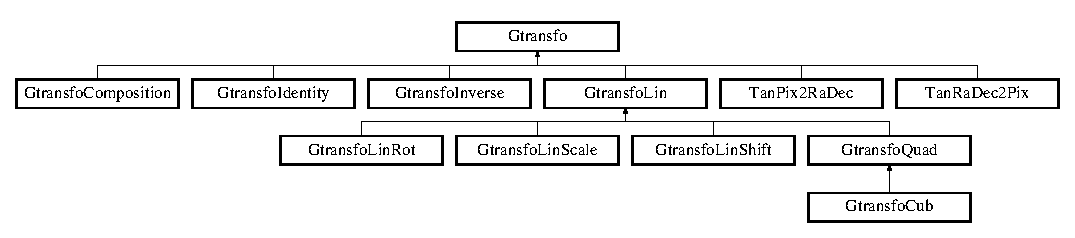
\includegraphics[height=2.7451cm]{class_gtransfo}
\end{center}
\end{figure}
\subsubsection*{Public Methods}
\begin{CompactItemize}
\item 
\index{apply@{apply}!Gtransfo@{Gtransfo}}\index{Gtransfo@{Gtransfo}!apply@{apply}}
virtual void {\bf apply} (const double Xin, const double Yin, double \&Xout, double \&Yout) const=0\label{class_gtransfo_a0}

\item 
\index{apply@{apply}!Gtransfo@{Gtransfo}}\index{Gtransfo@{Gtransfo}!apply@{apply}}
void {\bf apply} (const {\bf Point} \&Pin, {\bf Point} \&Pout) const\label{class_gtransfo_a1}

\begin{CompactList}\small\item\em applies the tranfo to Pin and writes into Pout. Is indeed virtual.\item\end{CompactList}\item 
\index{apply@{apply}!Gtransfo@{Gtransfo}}\index{Gtransfo@{Gtransfo}!apply@{apply}}
{\bf Point} {\bf apply} (const {\bf Point} \&Pin) const\label{class_gtransfo_a2}

\item 
\index{dump@{dump}!Gtransfo@{Gtransfo}}\index{Gtransfo@{Gtransfo}!dump@{dump}}
virtual void {\bf dump} (ostream \&stream=cout) const=0\label{class_gtransfo_a3}

\begin{CompactList}\small\item\em dumps the transfo coefficients to stream.\item\end{CompactList}\item 
virtual double {\bf fit} (const Star\-Match\-List \&List, const Gtransfo $\ast$Prior\-Transfo=NULL, const Gtransfo $\ast$Posterior\-Transfo=NULL)=0
\begin{CompactList}\small\item\em fits a transfo to a list of star pairs (p1,p2).\item\end{CompactList}\item 
\index{operator()@{operator()}!Gtransfo@{Gtransfo}}\index{Gtransfo@{Gtransfo}!operator()@{operator()}}
{\bf Point} {\bf operator()} (const {\bf Point} \&In) const\label{class_gtransfo_a5}

\begin{CompactList}\small\item\em allows to write My\-Transfo(My\-Star).\item\end{CompactList}\item 
\index{ReduceCompo@{ReduceCompo}!Gtransfo@{Gtransfo}}\index{Gtransfo@{Gtransfo}!ReduceCompo@{Reduce\-Compo}}
virtual Gtransfo$\ast$ {\bf Reduce\-Compo} (const Gtransfo $\ast$Right) const\label{class_gtransfo_a6}

\begin{CompactList}\small\item\em allow composition of transformations regardless of their actual types.see {\bf Gtransfo\-Compose}() {\rm (p.\,\pageref{gtransfo_h_a1})} for a user callable entry.\item\end{CompactList}\item 
\index{Clone@{Clone}!Gtransfo@{Gtransfo}}\index{Gtransfo@{Gtransfo}!Clone@{Clone}}
virtual Gtransfo$\ast$ {\bf Clone} () const=0\label{class_gtransfo_a7}

\begin{CompactList}\small\item\em returns a copy (allocated by new) of the transformation.\item\end{CompactList}\item 
\index{Jacobian@{Jacobian}!Gtransfo@{Gtransfo}}\index{Gtransfo@{Gtransfo}!Jacobian@{Jacobian}}
virtual double {\bf Jacobian} (const double x, const double y) const\label{class_gtransfo_a8}

\begin{CompactList}\small\item\em returns the local jacobian.\item\end{CompactList}\item 
virtual void {\bf Derivative} (const {\bf Point} \&Where, {\bf Gtransfo\-Lin} \&Der, const double Step=0.01) const
\begin{CompactList}\small\item\em Computes the local Derivative of a transfo. Step is used for numerical derivation.\item\end{CompactList}\item 
\index{LinearApproximation@{LinearApproximation}!Gtransfo@{Gtransfo}}\index{Gtransfo@{Gtransfo}!LinearApproximation@{Linear\-Approximation}}
virtual {\bf Gtransfo\-Lin} {\bf Linear\-Approximation} (const {\bf Point} \&Where, const double step=0.01) const\label{class_gtransfo_a10}

\begin{CompactList}\small\item\em linear (local) approximation.\item\end{CompactList}\item 
\index{TransformErrors@{TransformErrors}!Gtransfo@{Gtransfo}}\index{Gtransfo@{Gtransfo}!TransformErrors@{Transform\-Errors}}
virtual void {\bf Transform\-Errors} (const {\bf Point} \&Where, const double $\ast$VIn, double $\ast$VOut) const\label{class_gtransfo_a11}

\begin{CompactList}\small\item\em transform errors (represented as double[3] in order V(xx),V(yy),Cov(xy)).\item\end{CompactList}\item 
virtual Gtransfo$\ast$ {\bf Inverse\-Transfo} (const double Precision, const {\bf Frame} \&Region) const
\begin{CompactList}\small\item\em returns an inverse transfo.\item\end{CompactList}\item 
virtual Gtransfo$\ast$ {\bf Rough\-Inverse} (const {\bf Frame} \&Region) const
\begin{CompactList}\small\item\em Rough inverse.\item\end{CompactList}\item 
\index{Npar@{Npar}!Gtransfo@{Gtransfo}}\index{Gtransfo@{Gtransfo}!Npar@{Npar}}
virtual int {\bf Npar} () const\label{class_gtransfo_a14}

\begin{CompactList}\small\item\em returns the number of parameters (to compute chi2's).\item\end{CompactList}\item 
\index{~Gtransfo@{$\sim$Gtransfo}!Gtransfo@{Gtransfo}}\index{Gtransfo@{Gtransfo}!~Gtransfo@{$\sim$Gtransfo}}
virtual {\bf $\sim$Gtransfo} ()\label{class_gtransfo_a15}

\end{CompactItemize}


\subsubsection{Detailed Description}
a virtual (interface) class for geometric transformations.

We implement here One Gtransfo interface class, and actual derived classes. Composition in the usual (mathematical) sense is provided using {\bf Gtransfo\-Compose}() {\rm (p.\,\pageref{gtransfo_h_a1})}, and some classes (e.g. {\bf Gtransfo\-Lin} {\rm (p.\,\pageref{class_gtransfolin})}) handle a $\ast$ operator. Generic inversion by iteration exists, but it is at least 10 times slower than the corresponding \char`\"{}direct transformation\char`\"{}. If a transfo has an analytical inverse, then providing Inverse\-Transfo is obviously a very good idea. Before resorting to Inverse\-Transfo, consider using Star\-Match\-List::Inverse\-Transfo(). {\bf Gtransfo\-Lin::invert}() {\rm (p.\,\pageref{class_gtransfolin_a2})} and {\bf Tan\-Pix2Ra\-Dec::invert}() {\rm (p.\,\pageref{class_tanpix2radec_a7})} exist. The classes also provide derivation and linear approximation. 



\subsubsection{Member Function Documentation}
\index{Gtransfo@{Gtransfo}!Derivative@{Derivative}}
\index{Derivative@{Derivative}!Gtransfo@{Gtransfo}}
\paragraph{\setlength{\rightskip}{0pt plus 5cm}void Gtransfo::Derivative (const {\bf Point} \& {\em Where}, {\bf Gtransfo\-Lin} \& {\em Derivative}, const double {\em Step} = 0.01) const\hspace{0.3cm}{\tt  [virtual]}}\hfill\label{class_gtransfo_a9}


Computes the local Derivative of a transfo. Step is used for numerical derivation.

the Derivative is represented by a {\bf Gtransfo\-Lin} {\rm (p.\,\pageref{class_gtransfolin})}, in which (hopefully), the offset terms are zero. Derivative should  transform a vector of offsets into a vector of offsets. 

Reimplemented in {\bf Gtransfo\-Identity} {\rm (p.\,\pageref{class_gtransfoidentity_a7})}, {\bf Gtransfo\-Lin} {\rm (p.\,\pageref{class_gtransfolin_a5})}, and {\bf Gtransfo\-Quad} {\rm (p.\,\pageref{class_gtransfoquad_a9})}.\index{Gtransfo@{Gtransfo}!InverseTransfo@{InverseTransfo}}
\index{InverseTransfo@{InverseTransfo}!Gtransfo@{Gtransfo}}
\paragraph{\setlength{\rightskip}{0pt plus 5cm}Gtransfo $\ast$ Gtransfo::Inverse\-Transfo (const double {\em Precision}, const {\bf Frame} \& {\em Region}) const\hspace{0.3cm}{\tt  [virtual]}}\hfill\label{class_gtransfo_a12}


returns an inverse transfo.

Precision and Region refer to the \char`\"{}input\char`\"{} side of this,  and hence to the output side of the returned Gtransfo. 

Reimplemented in {\bf Gtransfo\-Lin} {\rm (p.\,\pageref{class_gtransfolin_a14})}, {\bf Gtransfo\-Quad} {\rm (p.\,\pageref{class_gtransfoquad_a8})}, {\bf Tan\-Pix2Ra\-Dec} {\rm (p.\,\pageref{class_tanpix2radec_a9})}, and {\bf Tan\-Ra\-Dec2Pix} {\rm (p.\,\pageref{class_tanradec2pix_a7})}.\index{Gtransfo@{Gtransfo}!RoughInverse@{RoughInverse}}
\index{RoughInverse@{RoughInverse}!Gtransfo@{Gtransfo}}
\paragraph{\setlength{\rightskip}{0pt plus 5cm}Gtransfo $\ast$ Gtransfo::Rough\-Inverse (const {\bf Frame} \& {\em Region}) const\hspace{0.3cm}{\tt  [virtual]}}\hfill\label{class_gtransfo_a13}


Rough inverse.

Stored by the numerical inverter to guess starting point  for the trials. Just here to enable overloading. 

Reimplemented in {\bf Tan\-Pix2Ra\-Dec} {\rm (p.\,\pageref{class_tanpix2radec_a8})}, and {\bf Tan\-Ra\-Dec2Pix} {\rm (p.\,\pageref{class_tanradec2pix_a6})}.\index{Gtransfo@{Gtransfo}!fit@{fit}}
\index{fit@{fit}!Gtransfo@{Gtransfo}}
\paragraph{\setlength{\rightskip}{0pt plus 5cm}double Gtransfo::fit (const Star\-Match\-List \& {\em List}, const Gtransfo $\ast$ {\em Prior\-Transfo} = NULL, const Gtransfo $\ast$ {\em Posterior\-Transfo} = NULL)\hspace{0.3cm}{\tt  [pure virtual]}}\hfill\label{class_gtransfo_a4}


fits a transfo to a list of star pairs (p1,p2).

After the fit this(Prior\-Transfo(p1)) yields approximately Posterior\-Transfo(p2). The returned value is the chi2. 

Reimplemented in {\bf Gtransfo\-Identity} {\rm (p.\,\pageref{class_gtransfoidentity_a2})}, {\bf Gtransfo\-Lin} {\rm (p.\,\pageref{class_gtransfolin_a9})}, {\bf Gtransfo\-Lin\-Shift} {\rm (p.\,\pageref{class_gtransfolinshift_a2})}, {\bf Gtransfo\-Lin\-Rot} {\rm (p.\,\pageref{class_gtransfolinrot_a2})}, {\bf Gtransfo\-Quad} {\rm (p.\,\pageref{class_gtransfoquad_a5})}, {\bf Gtransfo\-Cub} {\rm (p.\,\pageref{class_gtransfocub_a6})}, {\bf Tan\-Pix2Ra\-Dec} {\rm (p.\,\pageref{class_tanpix2radec_a17})}, and {\bf Tan\-Ra\-Dec2Pix} {\rm (p.\,\pageref{class_tanradec2pix_a10})}.

The documentation for this class was generated from the following files:\begin{CompactItemize}
\item 
{\bf gtransfo.h}\item 
gtransfo.cc\end{CompactItemize}
